%%%%%%%%%%%%%%%%%%%%%%%%%%%%%%%%%%%%%%%%%%%%%%%%%%%%%%%%%%%%%%%%%%%%%%
% Problem statement
\begin{statement}[
  problempoints=30,
  timelimit=1 sekunda,
  memorylimit=512 MiB,
]{Lijepi}

\setlength\intextsep{-0.1cm}
\begin{wrapfigure}[5]{r}{0.23\textwidth}
\centering
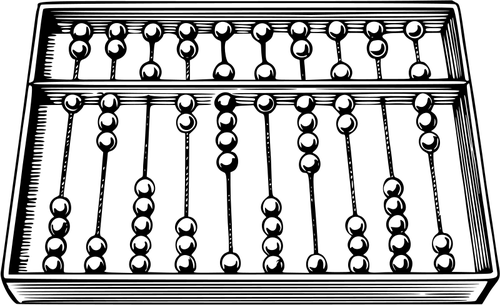
\includegraphics[width=0.23\textwidth]{img/abacus.png}
\end{wrapfigure}

Znate li bez kalkulatora izračunati koliko je $3+4$? A koliko je $23+67$? Svi
znaju da su odgovori na ova pitanja $7$ i $90$. Svi osim Filipa koji tvrdi da
su odgovori $34$ i $2367$. Očito je da on dva broja ne zbraja na ispravan način
već drugi broj \textit{lijepi} na kraj prvog da bi dobio svoje rješenje.

Neka je zadano $N$ izraza oblika $x+y$. Za svaki izraz odredite rješenje na
Filipov način, a onda na pravi način zbrojite tako dobivena rješenja.

%%%%%%%%%%%%%%%%%%%%%%%%%%%%%%%%%%%%%%%%%%%%%%%%%%%%%%%%%%%%%%%%%%%%%%
% Input
\subsection*{Ulazni podaci}
U prvom je retku prirodan broj $N$ $(1 \le N \le 10)$ iz teksta zadatka. \\
U sljedećih su $N$ redaka po dva prirodna broja $x$ i $y$ manja ili jednaka
milijardu koji opisuju izraz oblika $x+y$ iz teksta zadatka.

%%%%%%%%%%%%%%%%%%%%%%%%%%%%%%%%%%%%%%%%%%%%%%%%%%%%%%%%%%%%%%%%%%%%%%
% Output
\subsection*{Izlazni podaci}
U jedini redak ispišite ukupan zbroj $N$ brojeva dobivenih na Filipov način.

%%%%%%%%%%%%%%%%%%%%%%%%%%%%%%%%%%%%%%%%%%%%%%%%%%%%%%%%%%%%%%%%%%%%%%
% Scoring
\subsection*{Bodovanje}
U test podacima ukupno vrijednima $18$ bodova vrijedit će da je $N=1$ te da su
$X$ i $Y$ dvoznamenkasti. \\
U test podacima ukupno vrijednima $22$ boda vrijedit će $1 \le X, Y \le 999$.

%%%%%%%%%%%%%%%%%%%%%%%%%%%%%%%%%%%%%%%%%%%%%%%%%%%%%%%%%%%%%%%%%%%%%%
% Examples
\subsection*{Probni primjeri}
\begin{tabularx}{\textwidth}{X'X'X}
\sampleinputs{test/lijepi.dummy.in.1}{test/lijepi.dummy.out.1} &
\sampleinputs{test/lijepi.dummy.in.2}{test/lijepi.dummy.out.2} &
\sampleinputs{test/lijepi.dummy.in.3}{test/lijepi.dummy.out.3}
\end{tabularx}

\textbf{Pojašnjenje drugog probnog primjera:} \\
Prema Filipu, rješenje prvog izraza je $3412$, rješenje drugog $1137$, a
rješenje trećeg $4291$. Ukupan zbroj tih brojeva je $8840$.

%%%%%%%%%%%%%%%%%%%%%%%%%%%%%%%%%%%%%%%%%%%%%%%%%%%%%%%%%%%%%%%%%%%%%%
% We're done
\end{statement}

%%% Local Variables:
%%% mode: latex
%%% mode: flyspell
%%% ispell-local-dictionary: "croatian"
%%% TeX-master: "../hio.tex"
%%% End:
